\section{Outlier Detection}
An \textbf{outlier} (anomaly) is an observation that does not fit the distribution of the data for normal instances. In contrast, \textbf{noise} refers to random errors, typically caused by measurement imprecision, and does not produce unusual values.

\textbf{Outlier} (or \textbf{anomaly}) \textbf{detection} aims to identify unusual data points in a dataset, which can provide valuable insights across many applications.

An \textbf{anomaly detection technique} can be
\begin{itemize}
    \item \textbf{unsupervised:} anomalies are the points that do not fit well or that distort the model;
    \item \textbf{supervised:} anomalies are treated as a rare class, which requires labelled training data.
\end{itemize}
When the ground truth of anomalies is available, we can frame a classification problem to unveil outliers: here we can use ensembles, SVM, DNN, and similar models.
\subsection{Naive Approaches}
\subsubsection{Visual Approaches}

\textbf{Visual techniques} may detect outliers in a dataset. Common methods include:

\begin{itemize}
    \item \textbf{Boxplots:} outliers appear as individual points outside the \textit{whiskers} of the plot.
    \item \textbf{Scatter plots:} helps to identify outliers in 2D or 3D by visual inspection.
\end{itemize}

\textbf{Limitations:} they do not return explicit numerical values for outliers and rely on human interpretation.

\subsubsection{Inter-Quartile Range (IQR)}

\textbf{IQR} is a robust statistic used to identify outliers in a univariate distribution. Given \( Q_1 \) and \( Q_3 \) are the first and third quartiles, respectively, it is defined as:
\begin{equation}
\text{IQR} = Q_3 - Q_1    
\end{equation}
A data point \( x \) is considered an outlier if:
\begin{equation}
x < Q_1 - k \cdot \text{IQR} \quad \text{or} \quad x > Q_3 + k \cdot \text{IQR}    \qquad (k = 1.5 \text{ typically})
\end{equation}
In a boxplot, the \textit{whiskers} represent the data within the acceptable range, while any point beyond the whiskers is plotted as an individual outlier.

\subsubsection{Histogram-Based Outlier Score (HBOS)}

\textbf{HBOS} is an unsupervised anomaly detection method that \textbf{assumes feature independence}. It \textbf{estimates the density} of each feature individually by building histograms and identifies outliers as points with low estimated density.

\begin{itemize}
  \item For each feature, a univariate histogram is constructed:
    \begin{itemize}
      \item For \textbf{categorical data}: count the occurrences of each category.
      \item For \textbf{numerical data}: use binning methods such as \textit{equal-width} or \textit{equal-frequency}.
    \end{itemize}
  \item The frequency (relative count) in each bin is used as a proxy for density.
  \item Histograms are normalized so that densities are in the range $[0, 1]$.
  \item Given $d$ number of features, and $hist_i(p)$ the normalized frequency of the value of feature $i$ in the bin containing the data point $p$, we have:
  \begin{equation}
  HBOS(p) = \sum_{i=1}^{d} \log\left(\frac{1}{hist_i(p)}\right)      
  \end{equation}
\end{itemize}
\textbf{Pros:} efficient and scalable, especially for high-dimensional data.

\textbf{Cons:} relies heavily on the independence assumption between features.

\subsection{Statistical Approaches}
\textbf{Statistical approaches} model the normal class using \textbf{probability distributions}, assigning a probability value to each instance based on how likely it is to be generated from the distribution: outliers are those with low probability.

These methods rely on statistical tests that depend on the data distribution, its parameters (mean, variance, etc.), and an expected number of outliers (confidence limit). A key challenge is identifying the correct distribution, as real datasets often contain a mix of distributions. Additionally, these approaches are sensitive to the number of attributes.
\begin{itemize}
    \item \textit{Pros:} strong mathematical foundation, efficient, and effective when the distribution is known.
    \item \textit{Cons:} The data distribution is often unknown, and estimating it in high dimensions is difficult. Assumptions may be incorrect, and anomalies can distort distribution parameters. These methods are also inherently global.
\end{itemize}

\paragraph{Grubbs' Test (Model-Free, Global, Score)}
\textbf{Grubbs' Test} (\textbf{\ref{grubbs}}) detects outliers in a univariate dataset, under the assumption that the data follows a normal distribution. It identifies one outlier at a time and removes it from the dataset through a statistical hypothesis test:

\begin{itemize}
    \item Null hypothesis $H_0$: \textit{There are no outliers in the dataset.}
    \item Alternative hypothesis $H_A$: \textit{There is at least one outlier in the dataset.}
\end{itemize}

\begin{equation}\label{grubbs}
    G = \frac{\max |X_i - \bar{X}|}{s} \quad \bar{X} = \frac{1}{N} \sum_{i=1}^{N} X_i \text{ mean, }s = \sqrt{\frac{1}{N-1} \sum_{i=1}^{N} (X_i - \bar{X})^2} \text{ std dev.}
\end{equation}
\begin{itemize}
    \item $X_i$ is an individual observation in the dataset;
\end{itemize}

This statistic measures the distance between the most extreme value in the dataset and the sample mean, scaled by the standard deviation. The null hypothesis is rejected at significance level $\alpha$ if:
\begin{equation}
    G > \frac{N - 1}{\sqrt{N}} \cdot \sqrt{ \frac{t^2_{\alpha/N,\, N - 2}}{N - 2 + t^2_{\alpha/N,\, N - 2}} }
\end{equation}
\begin{itemize}
    \item $N$ is the total number of observations in the dataset.
    \item $t_{\alpha/N,\, N - 2}$ is the critical value from the $t$-distribution;
    \item $\alpha$ is the chosen significance level (e.g., $0.05$);
    \item $N - 2$ is the degrees of freedom for the $t$-distribution;
    \item $\alpha/N$ accounts for the Bonferroni correction, adjusting for multiple comparisons.
\end{itemize}

\textit{Note:} it is a one-sided test. To perform a two-sided test, the critical value should be computed using $\alpha/(2N)$ instead of $\alpha/N$.


\paragraph{Likelihood}
\textbf{Likelihood} assumes the dataset as a mixture of two probability distributions: $M$ (majority) and $A$ (anomalous), such that $D = (1-\lambda)M + \lambda A$. Initially, all points belong to $M$. Given $L_t(D)$ as the log-likelihood at time $t$, each data point $x_t$ is tested by temporarily moving it to $A$ and evaluating:

\begin{itemize}
    \item Compute the new log-likelihood $L_{t+1}(D)$.
    \item Calculate $\Delta = L_t(D) - L_{t+1}(D)$.
    \item If $\Delta > c$ (a user-defined threshold), $x_t$ is classified as an outlier and remains in $A$; otherwise, it returns to $M$.
\end{itemize}

\subsection{Deviation-Based Approaches}
Outliers are data points that deviate significantly from the overall structure of a dataset. Their removal typically reduces the dataset's variance. \textbf{Deviation-based approaches} build on this idea by assuming that outliers are the most extreme elements. A standard method involves the following components: a set of items $I$, a dissimilarity function $D$, and a cardinality function $C$ such that $I_1 \subset I_2 \Rightarrow C(I_1) < C(I_2)$ for all $I_1, I_2 \subseteq I$. The \textbf{smoothing factor} of a subset $I_j \subset I$ is defined as:
\begin{equation}
    SF(I_j) = C(I \setminus I_j) \cdot (D(I) - D(I \setminus I_j))
\end{equation}
This measures the decrease in dissimilarity when $I_j$ is removed, weighted by the size of the remaining set. The \textbf{exception set} $I_x \subset I$ is the subset that maximizes the smoothing factor:
\begin{equation}
    SF(I_x) \geq SF(I_j) \quad \forall I_j \subset I
\end{equation}
Intuitively, the exception set consists of the smallest group of items whose removal leads to the largest drop in dissimilarity: i.e., the outliers.

This approach does not assume any underlying distribution. While the naive solution has exponential complexity $O(2^n)$ for $n$ items, practical implementations use heuristics such as random sampling or best-first search. The method outputs a binary labeling of outliers.


\subsection{Depth-Based Approaches}
\begin{wrapfigure}{r}{0.4\textwidth}
    \centering
    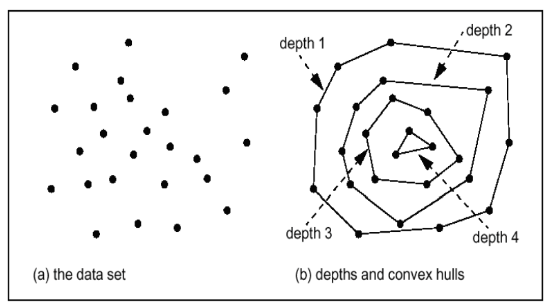
\includegraphics[width=\linewidth]{img/depth_based_od.png}
    \caption{depth-based detection.}\label{fig:depth-od}
\end{wrapfigure}
\textbf{Depth-based approaches} search for outliers at the borders of the data space. The data is organized into convex hull layers, with outliers lying in the outermost layers and normal points in the center, located in the innermost layers.

As shown in \textbf{Figure \ref{fig:depth-od}}, the points on the convex hull of the full dataset have depth 1. Points in the convex hull of the dataset obtained by removing those with depth 1 have depth 2, and so on. After calculating a certain number of convex hulls, points with a depth smaller than a user-defined threshold \(k\) are considered outliers. By default, the algorithm provides a binary classification (outlier or not), but it can be modified to return the depth of each point instead of a 0/1 classification. This method, however, is generally efficient only for two- or three-dimensional spaces.

Another depth-based method is the \textbf{Elliptic Envelope} algorithm which identifies the center of the data samples and draws an ellipsoid around it, creating an imaginary boundary around the dataset. Instances inside the envelope are considered normal, while those outside are flagged as outliers. This algorithm performs best on data with a Gaussian distribution.

\subsection{Proximity-Based Approaches}
\subsubsection{Distance-Based Approaches}
\paragraph{K-th Nearest Neighbor}
Outlier detection algorithms that use \( k \)-NN distances to score data can follow two approaches: either a simple \textbf{nested-loop} structure, where a sequential scan computes the \( k \)-NNs of each instance, or a \textbf{partition-based} approach, where data is first partitioned into micro clusters and information is aggregated for each partition. This allows pruning of micro clusters that cannot qualify when searching for the \( k \)-NNs of a point. Another common algorithm uses two parameters: a radius \( \varepsilon \) and a fraction \( \pi \in [0,1] \). A point \( p \) is considered an outlier if at most a fraction \( \pi \) of all other points have a distance to \( p \) less than \( \varepsilon \) (i.e., \( p \) is close to very few points). Formally, the set of outliers is computed as:
\begin{equation}
    \textit{OutlierSet}(\varepsilon, \pi) = \left\{ p \mid \dfrac{\#\{q \in D \mid \textit{dist}(p,q) < \varepsilon \}}{\# D} \leq \pi \right\}
\end{equation}

Finally, outliers can be identified using the \textbf{in-degree number}. Given a dataset, the \( k \)-NN graph is constructed: each vertex is a data point, and each directed edge between two vertices \( p \) and \( q \) means that \( q \) is one of \( p \)'s \( k \)-nearest neighbors. The in-degree of a point is calculated as the number of reverse \( k \)-NNs (R$k$-NN), i.e., the number of points that have it as a neighbor. If a point has an in-degree lower than a user-defined threshold, it is declared an outlier. This algorithm outputs an outlier label.

\textbf{Pros:} very simple to implement. They do not require any training, as they are model-free.

\textbf{Cons:} because the outcome depends on distances, these approaches can be slow and are less accurate in high-dimensional spaces. They are also sensitive to the chosen hyperparameters and to variations in density.

\subsubsection{Density-Based Outlier Detection}

The density around an instance can be defined as $n/V(d)$, where $n$ represents the number of instances within a specified distance, and $V(d)$ is the neighborhood volume. Since $V(d)$ stays constant for any fixed $d$, density is commonly represented by $n$ alone once $d$ is chosen. Outliers lie in low-density regions, and their anomaly score is the inverse of the density around them (or the inverse of the distance to the $k^{th}$ neighbor, or the inverse of the average distance to the $k$ neighbors). This approach breaks down when a dataset contains regions of varying density, the same difficulty seen with DBSCAN.

The \textbf{average relative density} can be used. For a point $x$ with $k$ neighbors, given $N(x,k)$ the $k$-nearest neighbors of $x$, this is calculated as:
\begin{equation}
    \textit{avg. relative density}(x,k) = \frac{\textit{density}(x,k)}{\sum_{y \in N(x,k)} \textit{density}(y,k)/|N(x,k)|} = \frac{1}{\text{distance with KNN}}
\end{equation}

\begin{algorithm}
\caption{Relative Density Outlier Score Algorithm}
\begin{algorithmic}[1]
\Require $k$ is the number of nearest neighbors
\ForAll{objects $\mathbf{x}$}
    \State Determine $N(\mathbf{x}, k)$, the $k$-nearest neighbors of $\mathbf{x}$.
    \State Determine $density(\mathbf{x}, k)$, the density of $\mathbf{x}$ using its nearest neighbors, i.e., the objects in $N(\mathbf{x}, k)$.
\EndFor
\ForAll{objects $\mathbf{x}$}
    \State Set the $outlier\ score(\mathbf{x}, k) = average\ relative\ density(\mathbf{x}, k)$ from Equation 10.7.
\EndFor
\end{algorithmic}
\end{algorithm}
\begin{wrapfigure}{r}{0.4\textwidth}
    \centering
    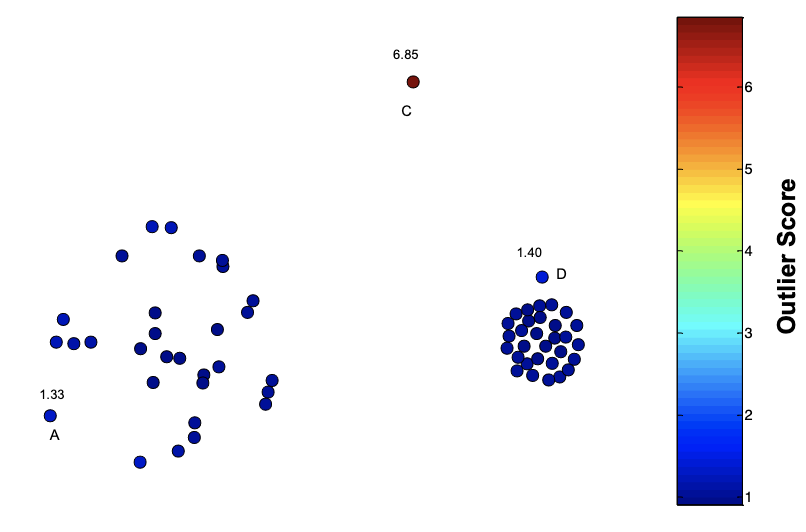
\includegraphics[width=\linewidth]{img/relative_density.png}
    \caption{$D$ is outlier, but is considered a normal point.}
    \label{fig:relative-dist}
\end{wrapfigure}
With this approach, a point's density depends on the density of its nearest neighbors. In datasets with regions of varying density, points in the lower-density regions are not misclassified as outliers. When a point sits far enough that its own density already looks high, its relative density stays high too. The method may still miss outliers that are anomalous only with respect to a very dense cluster, as shown in \textbf{Figure~\ref{fig:relative-dist}}.

\paragraph{Local Outlier Factor (LOF)}
\textbf{LOF} calculates, for each pair of points $(p,o)$ in the dataset, their \textbf{reachability distance} (as in OPTICS):
\begin{equation}
    \textit{reachability-dist}_k(p,o) = \max \left( \textit{k-dist}(o), \textit{dist}(p,o) \right)
\end{equation}
Then, each point is associated with its \textbf{local reachability density (LRD)}:
\begin{equation}
    \textit{LRD}_k(p) = \frac{1}{\dfrac{\sum_{o \in \textit{N}_k(p)} \textit{reachability-dist}_k(p,o)}{k}}
\end{equation}
Finally, the LOF is calculated as:
\begin{equation}
    \textit{LOF}_k(p) = \dfrac{\sum_{o \in N_{k(p)}} \dfrac{\textit{LRD}_k(o)}{\textit{LRD}_k(p)}}{k}
\end{equation}
If a point's LOF is close to 1, the point lies inside a cluster; if it is much greater than 1, the point is an outlier. The result depends on the chosen $k$, yet a larger $k$ does not necessarily raise the LOF.


\paragraph{Connectivity-Based Outlier Factor (COF)}
In regions of low density, LOF may fail to detect outliers unless we use a small $k$. A $k$ that is too small, though, may absorb outliers as normal points. A high-density set can represent a pattern, yet not every pattern needs to be high-density. One solution is the \textbf{Connectivity-based Outlier Factor (COF)}, useful when we want to treat isolation and density separately, its main difference from LOF. It uses \textbf{chaining distance} to characterise a point's nearest neighbor. The average chaining distance is:
\begin{equation}
    \textit{ac-dist}_{N_{k(p)}}(p) = \sum_{i=1}^{r-1} \dfrac{2(r-i)}{r(r-1)} \textit{CDS}_i
\end{equation}
where $r$ is the number of neighbors in $p$'s $k$-neighborhood, and $\textit{CDS}_i$ is the cost description sequence of removing the $i^{th}$ neighbor. The chaining distance of a point is the minimum total sum of the distances linking all neighbors, computed in practice through a graph-like structure. The COF is then the ratio between the average chaining distance of the point and the mean average chaining distance of the records in its $k$-NN:
\begin{equation}
    \textit{COF}_k(p) = \dfrac{|N_k(p)| \cdot \textit{ac-dist}_{N_{k(p)}}(p)}{\sum_{o \in N_{k(p)}} \textit{ac-dist}_{N_{k(o)}}(o)}
\end{equation}


\paragraph{Influenced Outlierness (INFLO)}

Previous methods cannot handle situations where clusters of varying densities are not well separated. \textbf{INFLO} incorporates symmetric neighborhood relationships: it considers both the nearest neighbors and the reverse nearest neighbors (the points for which $p$ is a neighbor), defining the \textbf{influence space} of a point $p$, denoted $kIS(p)$.

Density is the inverse of a point's $k$-distance. The INFLO score is then:
\begin{equation}
    \textit{INFLO}_k(p) = \dfrac{\sum_{o \in kIS(p)} \dfrac{\textit{den}(o)}{\# kIS(p)}}{\textit{den}(p)} \qquad\textit{den}(o) = \dfrac{1}{\textit{k-distance}(o)}
\end{equation}

\begin{wrapfigure}{r}{0.4\textwidth}
    \centering
    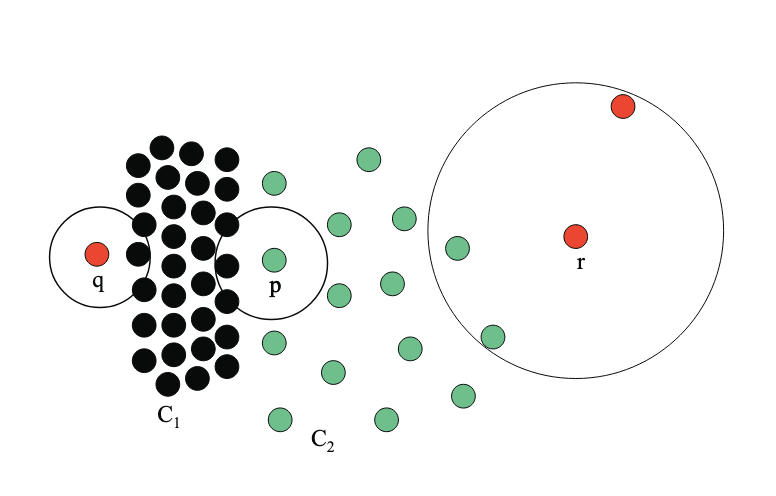
\includegraphics[width=\linewidth]{img/inflo.png}
    \caption{$q$ and $r$ have a lower LOF than $p$, despite $p$ not being an outlier in the sparse cluster on the right.}
    \label{fig:inflo}
\end{wrapfigure}

As with LOF, an INFLO score close to 1 marks a point inside a cluster, while a score significantly greater than 1 marks an outlier.

\paragraph{Pros} Density-based methods, like distance-based methods, are relatively simple to implement.

\paragraph{Cons} They are computationally expensive because they require calculating distances between all points in the dataset. Additionally, density becomes less meaningful as data dimensionality increases. These methods are also sensitive to the hyperparameters.


\subsection{Clustering-Based Approaches}

\textbf{Cluster-based outliers} are points that do not strongly fit into any cluster. For prototype-based clusters, this means the point is far from the prototype; for density-based clusters, it means the object has too low a density around it; for graph-based clusters, it means the point is not well connected.

Some clustering algorithms are already capable of separating points belonging to clusters from outliers (e.g., DBSCAN, OPTICS). One approach would be to simply apply these algorithms to the dataset, select the appropriate hyperparameters, and analyze the set of "noise" points returned by them. However, these are primarily clustering algorithms and are not optimized to detect outliers. As a result, sets of abnormal data objects may be mistakenly recognized as a cluster rather than as outliers.

\paragraph{Cluster-Based Local Outlier Factor (CBLOF)}
As with density-based outliers, we can use the \textbf{Cluster-Based Local Outlier Factor} (\textbf{CBLOF}). A clustering algorithm first finds the clusters in the dataset. Each cluster is then labelled either a \textbf{small cluster} (\textbf{SC}) or a \textbf{large cluster} (\textbf{LC}), using two parameters, $\alpha$ and $\beta$. Specifically, given the clustering $C = \{C_1, C_2, \dots, C_k \}$ such that $|C_1| \geq |C_2| \geq \dots \geq |C_k|$, a boundary $b$ is found if one of the following inequalities hold:
\begin{gather*}
    |C_1| + |C_2| + \dots + |C_b| \geq |D|*\alpha \\
    |C_b|/|C_{b+1}| \geq \beta
\end{gather*}
This means that all clusters up to the $b^{th}$ together hold $\alpha \%$ of the data points (first formula), or that the smallest large cluster is at least $\beta$ times larger than the largest small cluster (second formula).

The CBLOF depends on the size of the cluster the point belongs to and on the distance to the nearest large cluster. For a point in an LC, the outlier score is the cluster size times the distance to the cluster center. For a point in an SC, the score is the cluster size times the distance to the center of the closest LC.
\begin{equation}
    CBLOF(p) = \begin{cases}
        |C_i|*\min(d(p, C_j)),\; p \in C_i \land C_j \in LC & \text{if $C_i \in SC$} \\
        |C_i|*d(p, C_i) & \text{if $C_i \in LC, \,p \in C_i$}
    \end{cases}
\end{equation}

\paragraph{Pros} Cluster-based approaches are simple to implement and a variety of different algorithms exist.

\paragraph{Cons} A main issue is that the presence of outliers itself distorts the clustering. Choosing the appropriate hyperparameters and number of clusters is also hard when we have no prior knowledge of the data structure.

\subsection{High-Dimensional Approaches}
\begin{wrapfigure}{r}{0.4\textwidth}
    \centering
    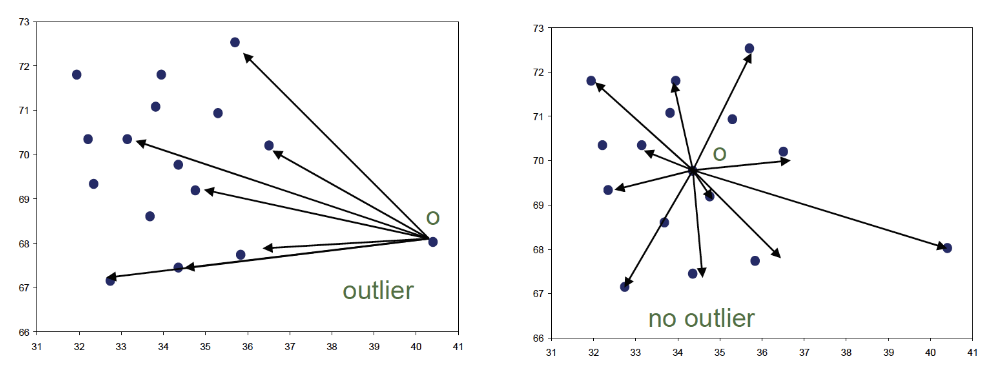
\includegraphics[width=\linewidth]{img/angle_based_od.png}
    \caption{angle-based outlier detection}
    \label{fig:angle-based}
\end{wrapfigure}
All approaches discussed previously share a significant limitation: they suffer from the curse of dimensionality, rendering them ineffective in high-dimensional spaces. The key issues include diminishing contrast between distances as dimensionality increases, data sparsity causing nearly all points to appear as outliers, and the concept of neighborhood becoming meaningless.

\paragraph{Angle-Based Outlier Degree (ABOD)}
\textbf{Angle-based outlier detection} analyzes the angles between pairs of distance vectors originating from the same point. In data clusters, angles vary widely, but for outliers, they tend to be similar.

For each point $p$, the angle between all pairs of points is calculated, and the angle spectrum is derived. A narrow spectrum results in a high outlier score, while a broad one indicates a low score.

The \textbf{ABOD} of $p$ is calculated as the variance of the angle spectrum weighted by the distances:
\begin{equation}
    \textit{ABOD}(p) = \underset{x,y \in D}{\mathrm{Var}} \left ( \dfrac{< \vec{xp}, \vec{yp} >}{\|\vec{xp}\|^2 \cdot \|\vec{yp}\|^2}  \right )
\end{equation}
A lower ABOD suggests a higher likelihood of being an outlier. The naive algorithm has a cost of $O(n^3)$, but it can be approximated using random sampling, calculating ABOD only for a subset of point pairs and filtering out points with a high lower bound of ABOD.

\paragraph{Grid-Based Subspace Outlier Detection}
\textbf{Grid-based subspace outlier detection} divides the $k$-dimensional data space into an equi-depth grid of $\Phi$ cells. The \textbf{sparsity coefficient} of a grid cell $C$ is defined as:
\begin{equation}
    S(C) = \dfrac{\textit{count}(C) - n (1/ \Phi)^k}{\sqrt{n(1/\Phi)^k (1-(1/\Phi)^k)}}
\end{equation}
where $\textit{count}(C)$ is the number of data points in $C$. If $S(C) < 0$, the count is lower than expected, and all points in that cell are labeled as outliers. The algorithm runs at a cost of $O(\Phi k)$.

The method stays quite simplistic: points in cells with low sparsity are labelled outliers directly, without further analysis. Its effectiveness therefore depends heavily on the grid's resolution and positioning.

\subsection{Ensemble-Based Approaches}

Ensemble-based methods combine the results of multiple techniques applied to the same dataset. For outlier detection, \textbf{feature bagging} (\textbf{FeaBag}) selects a set of outlier detection methods, each applied to a random subset of features from the original space. Each method assigns outlier scores, and the final score for each point is the average of these.

An extension of histogram-based outlier detection is the \textbf{Lightweight Online Detector of Anomalies} (\textbf{LODA}), which is particularly useful for real-time processing of large datasets. LODA approximates joint probabilities using one-dimensional histograms constructed from random projections of the input space. While individual histograms are weak for outlier detection, their combination yields effective results.


\subsection{Model-Based Approaches}
\paragraph{Isolation Forest}

The \textbf{Isolation Forest} is a specialized outlier detection model. It initializes multiple trees, each receiving a different random data sample. Each tree isolates points by recursively partitioning the data:

\begin{algorithm}
\caption{Isolation Forest Algorithm}
\begin{algorithmic}[1]
\State \textbf{Input:} Dataset $D = \{x_1, x_2, \dots, x_n\}$ 
\State \textbf{Output:} Outlier scores for each point
\For{each tree in the ensemble}
    \State Sample a subset from $D$
    \State Until tree construction completes:
        \State Select a random dimension
        \State Choose a random split value
        \State Create a separating hyperplane, dividing data into two subsets
        \State Recursively split each subset until stopping condition is met
\EndFor
\end{algorithmic}
\end{algorithm}

Outliers typically require fewer splits (lower tree depth) for isolation, while normal points need more splits (greater depth). Tree splitting can terminate at a fixed depth (10-20 levels) to prevent overfitting. The algorithm runs multiple times (e.g., 100 iterations), creating different trees that offer various perspectives on point isolation. Points consistently isolated with few splits across multiple trees are classified as outliers.

For new data points, only the isolation path needs to be calculated, making the model highly efficient. The outlier score for point $x$ in a dataset of size $n$ is:

\begin{equation}
    s(x, n) = 2^{\frac{-\mathrm{E}[h(x)]}{c(n)}}
\end{equation}

where $\mathrm{E}[h(x)]$ is the expected path length, and $c(n)$ is a scaling factor:

\begin{equation}
    c(n) = \begin{cases}
        1 & \text{if } n = 2 \\
        2 \cdot H(n-1) - \frac{2(n-1)}{n} & \text{if } n > 2 \\
        0 & \text{otherwise}
    \end{cases}
\end{equation}
\begin{wrapfigure}{r}{0.25\textwidth}
    \centering
    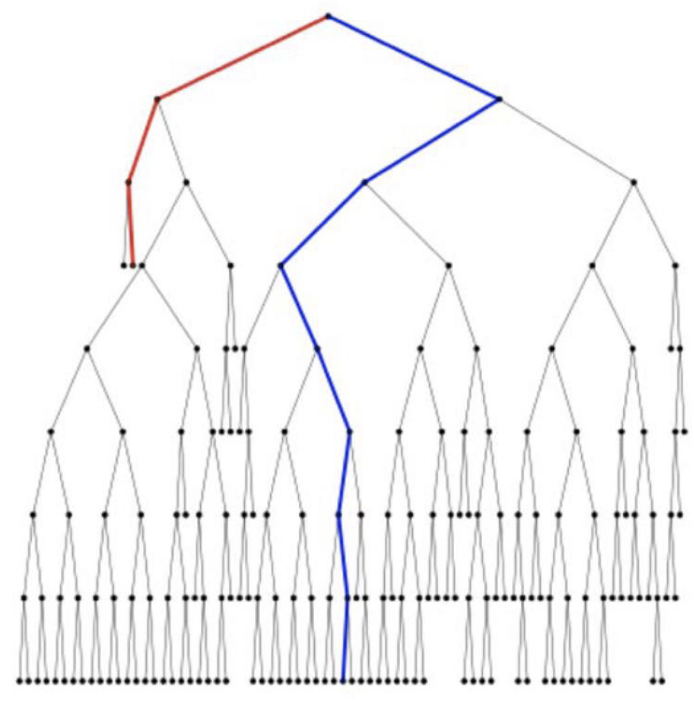
\includegraphics[width=\linewidth]{img/isolation_tree.png}
    \caption{red path: anomaly; blue path: normal point.}
    \label{fig:isolation-tree}
\end{wrapfigure}

with $H(i) = \ln(i) + \gamma$ representing the $i^{th}$ harmonic number and $\gamma \approx 0.577$ the Euler-Mascheroni constant.
Isolation Forests offer computational efficiency, parallelizability, and effectiveness with high-dimensional data. However, their scoring process may be inconsistent since space is always split along single dimensions. For bi-dimensional data with non-linear patterns, the axis-aligned splits may underperform, potentially requiring data transformation into grid-like structures for improved results.

\paragraph{Extended Isolation Forest}


The \textbf{extended isolation forest} model fixes a weakness of standard isolation forests: instead of choosing a single dimension, each tree randomly selects both a normal vector and an intercept that describe an angled hyperplane.

For each tree, we begin by drawing a random sample from the dataset. A random normal vector is chosen next, followed by a random intercept. From these, a separating hyperplane is placed at the chosen intercept value, splitting the data into two parts. The process repeats recursively, each new split isolating more data points, until the tree is complete. Tree construction stops when a predefined depth or condition is met, so that every data point ends up isolated in a leaf node. Again, the extended isolation forest is computationally efficient, parallelizable, and able to handle high-dimensional data; unlike the isolation forest, it has consistent scoring.

\begin{figure}
    \centering
    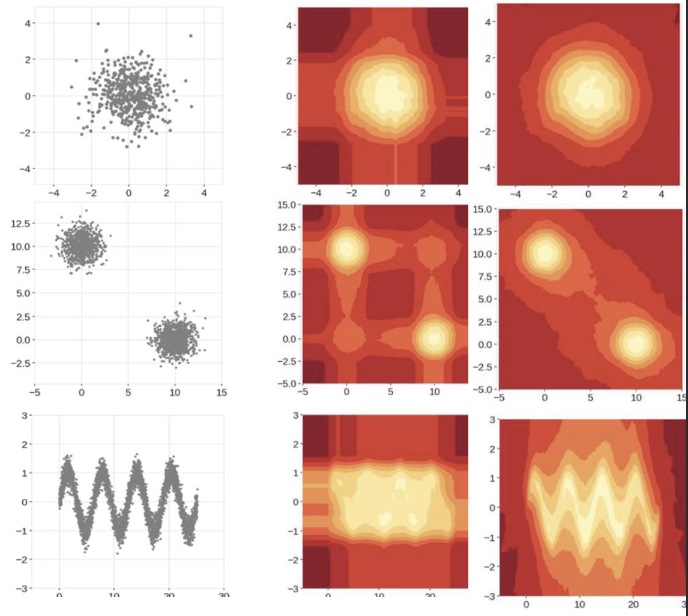
\includegraphics[width=0.4\linewidth]{img/isolation_forests.png}
    \caption{Isolation forests and Extended isolation forests, compared.}
    \label{fig:isolation-forests}
\end{figure}
